% This is samplepaper.tex, a sample chapter demonstrating the
% LLNCS macro package for Springer Computer Science proceedings;
% Version 2.20 of 2017/10/04
%
\documentclass[runningheads]{llncs}
%
\usepackage{comment}
\usepackage{graphicx}
\usepackage{amsmath}
\usepackage{footmisc}
\usepackage{array, boldline, makecell, booktabs}
\usepackage[utf8]{inputenc}
\usepackage[T1]{fontenc}
\addtolength{\parskip}{-0.5mm}
\newcolumntype{P}[1]{>{\centering\arraybackslash}p{#1}}
\newcolumntype{M}[1]{>{\centering\arraybackslash}m{#1}}

% Used for displaying a sample figure. If possible, figure files should
% be included in EPS format.
%
% If you use the hyperref package, please uncomment the following line
% to display URLs in blue roman font according to Springer's eBook style:
% \renewcommand\UrlFont{\color{blue}\rmfamily}

\begin{document}
%
\title{End-to-end Fine-grained Neural Entity Recognition of Patients, Interventions, Outcomes\thanks{Supported by HES-SO Valais-Wallis, Switzerland}} 
%
%\titlerunning{Abbreviated paper title}
% If the paper title is too long for the running head, you can set
% an abbreviated paper title here
%
\author{Anjani Dhrangadhariya\inst{1,2}\orcidID{0000-0003-1691-1338} \and
Gustavo Aguilar\inst{3}\orcidID{0000-0002-3028-7626} \and
Thamar Solorio\inst{3}\orcidID{0000-0002-3541-9405}
\and 
Roger Hilfiker\inst{4}\orcidID{0000-0001-8662-6116}
\and 
Henning Müller\inst{1,2}\orcidID{0000-0001-6800-9878}}
%
\authorrunning{A. Dhrangadhariya et al.}
% First names are abbreviated in the running head.
% If there are more than two authors, 'et al.' is used.
%
\institute{University of Geneva (UNIGE), Geneva, Switzerland \and
University of Applied Sciences Western Switzerland (HES-SO), Sierre, Switzerland
\email{anjani.dhrangadhariya@hevs.ch}\\ \and
University of Houston, Houston, Texas, USA\\
\and
School of Health Sciences, HES-SO Valais-Wallis, Leukerbad, Switzerland\\
}
%
\maketitle              % typeset the header of the contribution
%
\begin{abstract}
PICO recognition is an information extraction task for detecting parts of text describing Participant (P), Intervention (I), Comparator (C), and Outcome (O) (PICO elements) in clinical trial literature.
Each PICO description is further decomposed into finer semantic units.
For example, in the sentence `The study involved 242 adult men with back pain.', the phrase `242 adult men with back pain' describes the participant, but this coarse-grained description is further divided into finer semantic units.
The term `242' shows ``sample size'' of the participants, `adult' shows ``age'', `men' shows ``sex'', and `back pain' show the participant ``condition''.
Recognizing these fine-grained PICO entities in health literature is a challenging named-entity recognition (NER) task but it can help to fully automate systematic reviews (SR).
Previous approaches concentrated on coarse-grained PICO recognition but focus on the fine-grained recognition still lacks.
We revisit the previously unfruitful neural approaches to improve recognition performance for the fine-grained entities.
In this paper, we test the feasibility and quality of multitask learning (MTL) to improve fine-grained PICO recognition using a related auxiliary task and compare it with single-task learning (STL).
As a consequence, our end-to-end neural approach improves the state-of-the-art (SOTA) F1 score from 0.45 to 0.54 for the ``participant'' entity and from 0.48 to 0.57 for the ``outcome'' entity without any handcrafted features.
We inspect the models to identify where they fail and how some of these failures are linked to the current benchmark data.
%
\keywords{Named entity recognition  \and Health \and Evidence-based health.}
\end{abstract}
%
\section{Introduction}
\label{sec:introduction}
%
Systematic reviews (SR) are cornerstones of evidence-based medicine (EBM) and aim to answer clinically relevant questions with utmost objectivity, transparency, and reproducibility.
Primary relevance screening is a very resource-consuming process involving reviewers manually screening thousands of clinical trial abstracts for inclusion into an SR~\cite{khangura2012evidence}.
The criteria for including a study into an SR is decomposed into whether all or most predetermined PICO elements are present in the study~\cite{russell2009systematic}.
Machine learning (ML) algorithms can help automate the recognition of PICO elements from clinical trial studies by directly pointing the human reviewers to the correct PICO descriptions in a document.
However, the detected coarse-grained PICO descriptions (see Section~\ref{subsec:datasets}) are further delineated into fine-grained semantic units (see Figure~\ref{fig:coarsefineexample}).
%
\begin{figure}[ht]
    \centering
    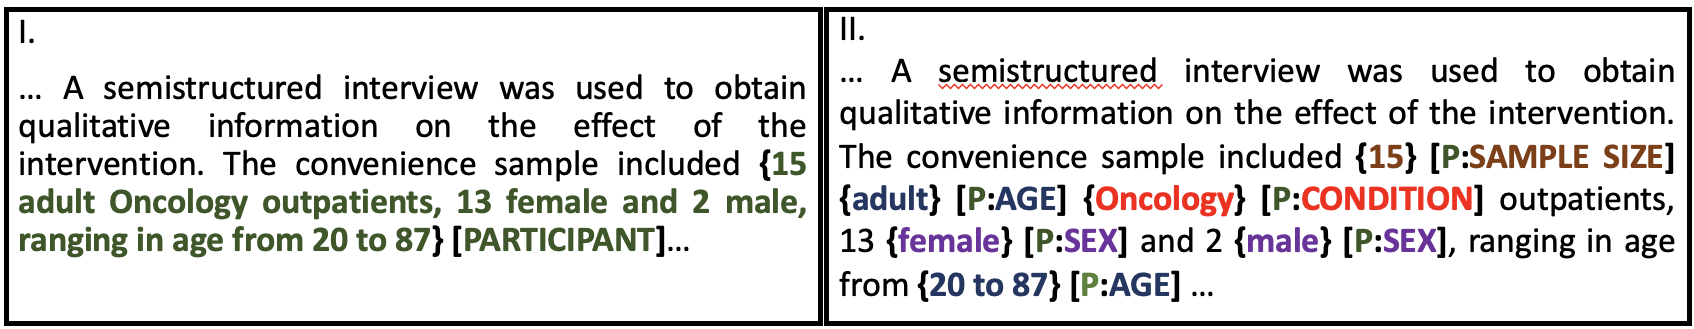
\includegraphics[scale=0.33]{figures/finecoarse1.png}
    \caption{Example of I. coarse-grained annotated participant span and II. further delineated fine-grained participant entities (P = Participant). }
    \label{fig:coarsefineexample}
\end{figure}
%
This means that even after a machine points a human reviewer to the correct coarse-grained PICO description, the reviewer requires to manually read and understand its finer aspects to screen the study for relevance. 
This leads to the semi-automation of the process.
Fully automating the relevance screening process requires identifying, delineating, and normalizing the fine-grained PICO mentions allowing for machine reasoning over the extracted semantic units.
Unlike in many biomedical journals, fine-grained PICO mentions in the broader health literature are neither clearly identified nor standardized as semantic units (e.g. naming conventions for interventions and outcome measurement) making it an even more tedious process for the reviewers~\cite{he2017semantics}.
This hampers machine reasoning over the semantic units leading to barriers for full automation.

In this work, we test and propose end-to-end neural attention models that require no hand-engineered features unlike the previous approaches and are trained to improve recognition of fine-grained PICO entities.
Our approach achieves state-of-the-art (SOTA) performance for fine-grained ``Participant'' and ``Outcome'' entity recognition.
In our approach, fine-grained PICO recognition was considered as a sequence labeling task for which two different setups were tested: single-task learning (STL) and multi-task learning (MTL).
We investigate if these model setups trained on the PICO benchmark corpus extend to reaching similar performance for an \textit{in-house} PICO-annotated corpus from the physical therapy domain (hereafter: physiotherapy corpus).
The key takeaway from the error analysis and corpus exploration is that the PICO benchmark corpus over-represents pharmaceutical entity labels leading to poor performance on any low-frequency entities especially the non-pharma entities coming from domains of physiotherapy, complementary therapies and in the more general health domain.
Automating PICO recognition is far more challenging compared to open-domain NER because there are disagreements even between human experts on the exact words that make up PICO elements.
Additionally, PICO recognition cannot be purely labeled as an NER task because ``Participant'' entities span entire sentences.
%
\section{Related work}
\label{sec:relatedwork}
%
Research towards automatic PICO recognition peaked with exploration of several methods including rule-based lexical approaches~\cite{dawes2007identification}, language models (LM)~\cite{boudin2010clinical}, support vector machines (SVMs)~\cite{boudin2010improving}, graphical models like CRF~\cite{chabou2018combination}, shallow neural (Multilayer Perceptrons) approaches~\cite{pmid20470429}, a combination of ML and rules~\cite{chabou2018combination} and deep neural approach like LSTMs~\cite{jin2018pico}. 
These studies, however, used small annotated corpora, heavy text pre-processing, and hand-engineered features.

The availability of a comparatively large, and probably the only PICO benchmark corpus (EBM-PICO corpus hereafter) from~\cite{nye2018corpus} with multi-grained (fine and coarse-grained) PICO annotations opened up possibilities to explore the neural models.
Nye \textit{et al.}~\cite{nye2018corpus} used this corpus to train baseline models using hand-engineered features for separately detecting fine- and coarse-grained entities.
Their baselines achieved a good performance on the coarse-grained PICO but a poor performance on the more difficult, semantic fine-grained entities.\footnote{https://ebm-nlp.herokuapp.com/}
SciBERT, through domain-adaptation, improved\footnote{https://paperswithcode.com/sota/participant-intervention-comparison-outcome} the overall coarse-grained PICO recognition for the EBM-PICO corpus~\cite{beltagy2019scibert}.
A few studies dived into the recognition of finer aspects of PICO but did not focus on all of them together.
For instance, the DNER (Disease NER)~\cite{zhang2020unlocking} neural model focused on disease-mention recognition,~\cite{xu2007extracting} concentrated on recognition of patient demographics (sex, sample size, disease) and~\cite{chung2009towards} explored recognition of different intervention arms from RCTs (randomized controlled trials).
Except~\cite{nye2018corpus}, prior work either focused on coarse-grained or sentence-level PICO recognition.
Fine-grained PICO recognition has not yet garnered as much attention as it should given its potential for fully automating the SR screening phase.

The focus of our work is to improve recognition of fine-grained PICO entities, test feasibility and competency of MTL models utilizing joint information from the fine- and coarse-entity annotation, and improve generalization by introducing inductive bias~\cite{caruana1997multitask}.
The work stands out because both PICO corpus and the current SOTA automation methods focus on the overall entity recognition but do not explore domain differences.
Both the MTL and STL models trained on the EBM-PICO benchmark corpus were used to evaluate fine-grained performance on the physiotherapy corpus. 
%
\section{Methodology}
\label{sec:methodology}
%
%This section describes our motivation for using the MTL approach, the datasets used, the end-to-end MTL system (refer Figure~\ref{fig:mtlsetup}), and its components.
%
\subsection{Multitask learning}
\label{subsec:mtl}
%
As fine-grained entities are nested under coarse-grained spans (see Figure~\ref{fig:coarsefineexample}), we assume both entity extractions as closely related tasks that can serve as mutual sources of inductive bias for each other.
This opens up the possibility to jointly training both tasks using the MTL approach~\cite{caruana1997multitask,ruder2017overview}.
MTL has previously shown to leverage performance on nested biomedical named-entities (NEs) for example for the GENIA corpus~\cite{fei2020dispatched}.
In contrast to an STL setup that requires a separate setup to recognize fine-grained and coarse-grained entities, an end-to-end MTL system jointly learns to recognize both by exploiting the similarities and differences between the task characteristics.
MTL opens up the possibility to improve recognition of poorly performing\footnote{https://ebm-nlp.herokuapp.com/\#Leaderboard} fine-grained recognition by sharing the hidden representation with the far better performing coarse-grained task.
For comprehensive details on the MTL algorithms in NLP read~\cite{ruder2017overview}.

In our MTL setup, fine-grained PICO recognition was considered as the main task and involved assigning each token in the input text with the fine-grained PICO class labels (see Table~\ref{table:coarsefineconcept}).
Coarse-grained recognition was considered as an auxiliary task and involved assigning each token in the input text with either 1 (``Participant'' or ``Intervention'' or ``Outcome'') or 0 (``No Label'').
For both tasks, 0 (``No Label'') was considered as the out-of-the-span or non-span label.
We began training simple models and sequentially added more layers to understand the improvement effect.
To probe the cumulative effect of the self-attention component on the tasks in the MTL setup two ablation experiments were performed~\cite{vaswani2017attention}.
%
\begingroup
\setlength{\tabcolsep}{5pt} % Default value: 6pt
\renewcommand{\arraystretch}{1.0}
\begin{table}[h!]
\begin{center}
\caption{Coarse-grained P (Participant), I (Intervention) and O (Outcome) labels are delineated into respective fine-grained labels. Annotation counts are shown in the table.}
\label{table:coarsefineconcept}
\begin{tabular}{ c  l  c  l  c  l  c } 
\Xhline{1pt}
& Participant & count & Intervention/Comparator & count  & Outcome & count  \\ 
\Xhline{1pt}
0 & No label & 124372 & No label & 120453 & No label & 115578\\ 
1 & Age & 708 & Surgical & 659  & Physical & 7215\\ 
2 & Sex & 157 & Physical & 1988 & Pain & 180\\
3 & Sample size & 661 & Drug & 4424 & Mortality & 261\\
4 & Condition & 3893 & Educational & 1328 & Side effect & 540\\
5 & & & Psychological & 62 & Mental & 1657\\
6 & & & Other & 323 & Other & 2064\\
7 & & & Control & 542 & & \\
\Xhline{1pt}
\end{tabular}
\end{center}
\end{table}
\endgroup
%
%
\subsection{Datasets}
\label{subsec:datasets}
%
\paragraph{EBM-PICO test set: }
%
We used the EBM-PICO corpus comprising $\sim$5000 coarse- and fine-grained PICO-annotated documents~\footnote{A single document consists of a title and an abstract.} to train and test the end-to-end system (see Figure~\ref{fig:coarsefineexample} and Table~\ref{table:coarsefineconcept}).
A part of the dataset was annotated by crowd-sourcing and a small part by medical experts.
It comes pre-divided into a training set comprising 4,993 documents and a test set comprising 191 that was used for evaluation.
More details about the dataset can be found in~\cite{nye2018corpus}.
%
\paragraph{Physiotherapy and Rehabilitation test set: }
%
An additional test set comprising 153 documents in an \textit{in-house} SR titled "Exercise and other non-pharmaceutical interventions for cancer-related fatigue in patients during or after cancer treatment: a SR incorporating an indirect-comparisons meta-analysis" was manually annotated by the first author using the annotation instructions\footnote{https://www.ncbi.nlm.nih.gov/pmc/articles/PMC6174533/bin/NIHMS988059-supplement-Appendix.pdf} available from~\cite{nye2018corpus,hilfiker2018exercise}.
The primary purpose of this additional test dataset was not to establish any inter-annotator agreement (IAA) but 1) to understand the complexity and noise encompassed in the multi-grained PICO annotation process, and 2) to test the feasibility of the proposed setups trained on the general medical (EBM-PICO) dataset to predict PICO classes for a corpus from physiotherapy and rehabilitation domains.
The vitality of this annotation exercise will be apparent in the discussion section (see Section~\ref{sec:results}).
IO (Inside, Outside) or raw labeling was used for both sequence labeling tasks.
%
\subsection{System components}\label{subsec:sys_comp}
%
\paragraph{1. Embeddings:}
%
Contextual representations like BERT, ULMFit, GPT encode rich syntactic and semantic information from the text into vectors eliminating the need for heavy feature engineering.
They also tackle the challenge of out-of-vocabulary (OOV) words using the WordPiece tokenizer and byte pair encoding (BPE)~\cite{devlin2018bert,joshi2019comparison}.
The proposed model setups used SciBERT to extract dense, contextual vectors $e_{t}$ from the encoded input text tokens $x_{t}$ at each time-step $t$.
%
\paragraph{2. Feature transformer:}
%
To encode long-term dependencies and learn a task-specific text structure from the input documents, the model stacked a single bidirectional LSTM (BiLSTM) layer on top of the embedding layer~\cite{hochreiter1997long}.
A forward LSTM ran from left-to-right (LTR) encoding the text into a $(\overrightarrow{h})$ vector using the current token embedding input $e_{t}$ and the previous hidden state $h_{t-1}$.
A backward LSTM does the same from right to left (RTL).
Both outputs were shallowly concatenated $([\overrightarrow{h}; \overleftarrow{h}])$ into $h_{t}$ and used as the input for the next layer.
%
\paragraph{3. Self-attention: }
%
Next, the model stacked a softmax-based multi-head self-attention layer that calculated for each token in the sequence a weighted average of the feature representation of all other tokens in the sequence~\cite{vaswani2017attention}.
Self-attention improves the signal-to-noise ratio by out-weighting important tokens.
Self-attention weights for each token were calculated by multiplying hidden representation $h_{t}$ with randomly initialized Query $q$ and Key $k$ weights, which were further multiplied with each other to obtain attention weighted vectors.
Finally, the obtained attention weights were multiplied with the Value (V) matrix which was obtained by multiplication between a randomly initialized weight matrix $v$ and $h_{t}$ finally obtaining scaled attention-weighted vectors $a_{t}$.
%
\paragraph{4. Decoder:}
%
The attention-weighted representation $a_{t}$ is either fed to a linear layer to predict the tag emission sequence followed by calculation of weighted cross-entropy loss or to a CRF layer along with the true tag sequence $y_{t}$.
CRF is a graph-based model suitable for learning tag sequence dependencies from the training set and it has shown to outperform softmax classifiers~\cite{huang2015bidirectional}.
%
\begin{figure}
    \centering
    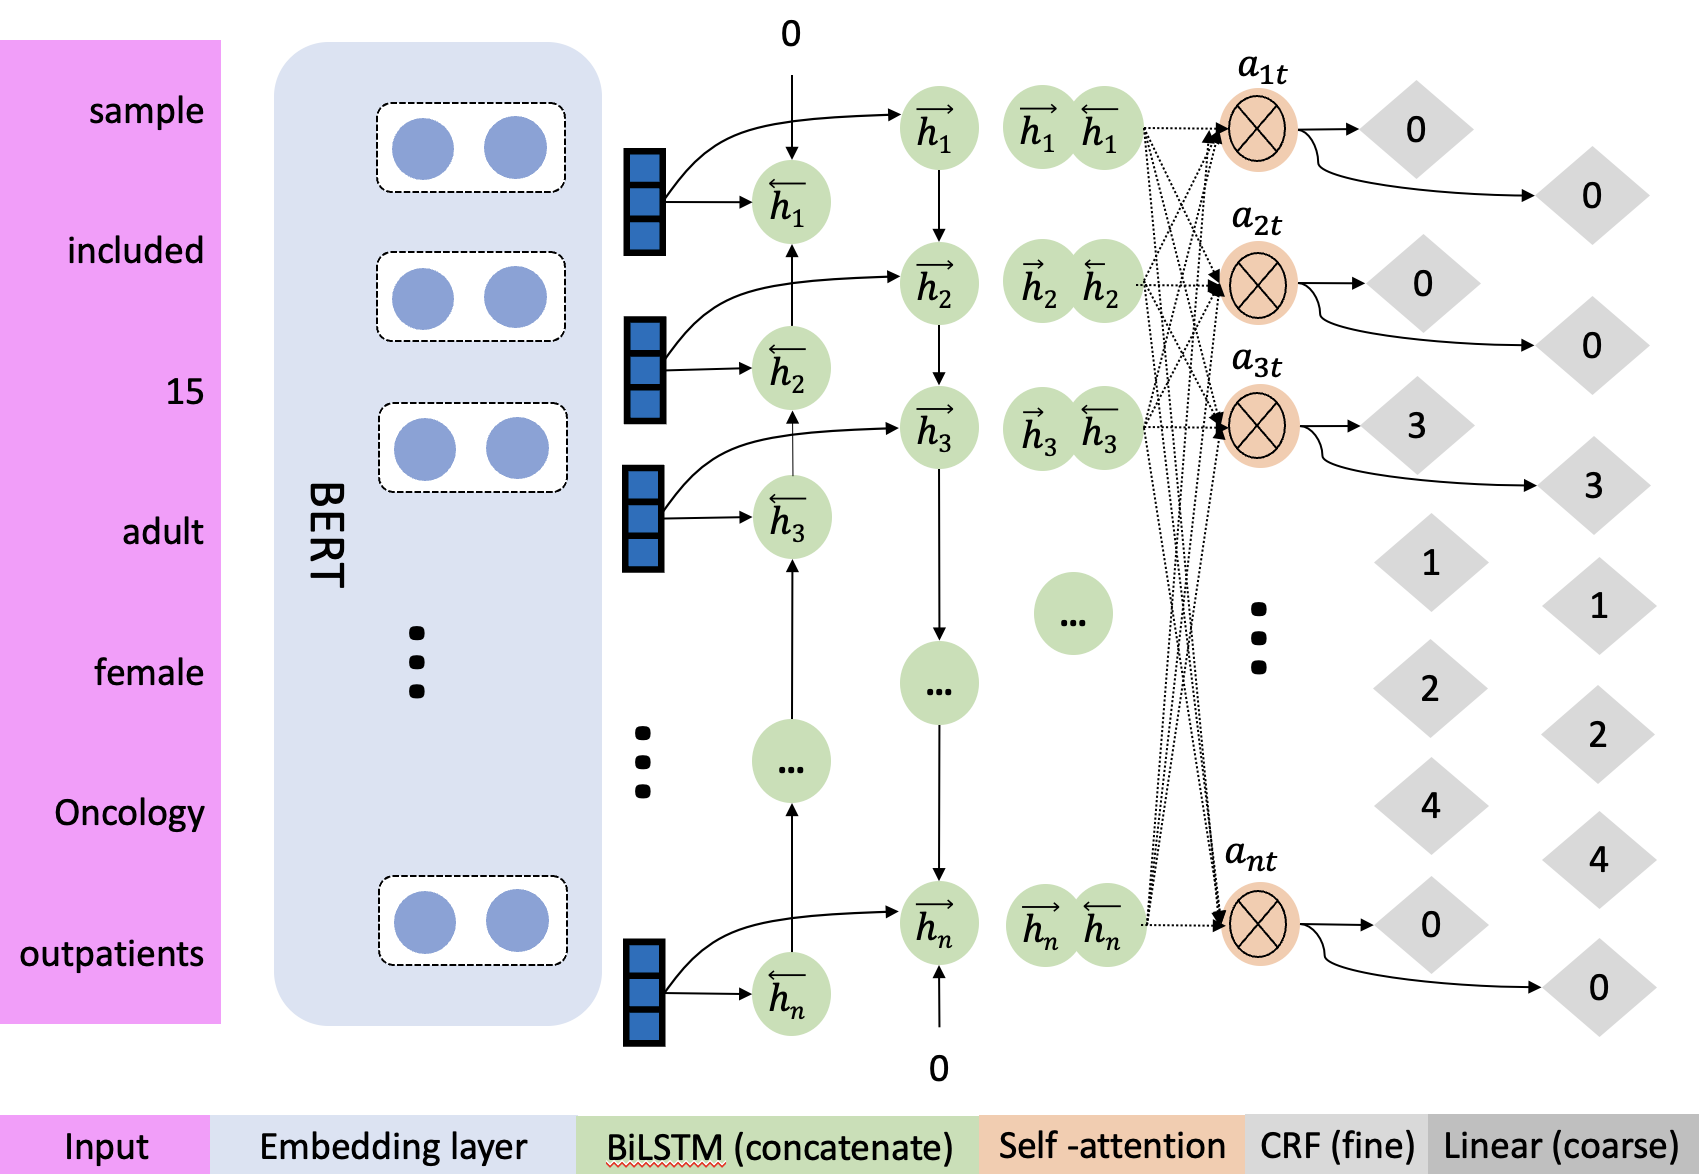
\includegraphics[scale=0.34]{figures/CLEF2021.png}
    \caption{The proposed end-to-end MTL approach with fine-grained recognition as the main-task and coarse-grained as the auxiliary task. Removing either of the CRF decoder heads gives the respective STL setup.}
    \label{fig:mtlsetup}
\end{figure}
%
%
\section{Experiments}
\label{sec:experiments}
%
To compare our proposed methodology on fine-grained PICO recognition, two strong baselines from Nye \textit{et al.} were used.
The baselines use a combination of n-grams, part-of-speech tags, and character embeddings as features and used them to separately train a logistic regression model and a neural LSTM-CRF.
To demonstrate the feasibility of the MTL approach for improving fine-grained recognition using the auxiliary coarse-grained task and to compare the performance of each MTL setup, exactly identical STL setups were used.
The setups are: 
\begin{comment}
The setups are detailed in Table~\ref{tab:exp_setup}.
Each setup stacks an embedding layer to encode the input text tokens followed by a feature transformer, a self-attention head applied to the transformed features, and finally an appropriate decoder which was either a linear layer or a linear layer followed by CRF decoder.
The setups are:

\begin{table}[h!]
    \centering
    \caption{The table shows seven experimental setups from I...VII with each system component (refer Section~\ref{subsec:sys_comp}) stacked on top of the other. SH = Single-head, MH = Multi-head, Lin = Linear layer, W CELoss = Weighted Cross Entropy loss.}
    \label{tab:exp_setup}
    \begin{tabular}{M{0.5cm}M{2cm}M{3cm}M{2.5cm}M{1.5cm}M{2cm}}
        \Xhline{1pt}
         & \multicolumn{3}{c}{Encoder} & Decoder & Loss \\
        \hline
         & Embeddings & Feature transformer & Attention &  & \\
        \Xhline{1pt}
        I & BERT & - & - & Lin & W CEloss\\
        II & BERT & LSTM & - & Lin, CRF &  CRF loss\\
        III & BERT & BiLSTM & - & Lin, CRF & CRF loss\\
        IV & BERT & LSTM & SH self-attention & Lin, CRF & CRF loss\\
        V & BERT & BiLSTM & SH self-attention & Lin, CRF & CRF loss\\
        VI & BERT & BiLSTM & MH self-attention & Lin, CRF & CRF loss\\
        VII & BERT & BiLSTM & MH self-attention & Lin & W CEloss\\
        \Xhline{1pt}
    \end{tabular}
\end{table}
\end{comment}
%
\paragraph{I. BERT Linear} setup includes a linear transformation layer stacked on top of the BERT\textsubscript{BASE} model followed by weight-balanced cross-entropy loss calculation.

\paragraph{II. BERT LSTM CRF} setup uses BERT\textsubscript{BASE} for feature extraction followed by an LSTM and a linear layer to generate emission probabilities that feed into the CRF decoder head that learns tag sequence dependencies and calculates loss. 

\paragraph{III. BERT BiLSTM CRF} setup is identical to setup II, but BiLSTM replaces the LSTM layer.

\paragraph{IV. BERT LSTM atten CRF} setup incorporates a single self-attention head.
Attention weights calculated by the attention head are applied to the output of the LSTM layer followed by a linear transformation to generate emission probabilities. These probabilities feed into the CRF decoder.

\paragraph{V. BERT BiLSTM atten CRF} setup is identical to the setup IV, but BiLSTM replaces the LSTM layer.

\paragraph{VI. BERT BiLSTM Multihead atten CRF} setup differs from setup V in how attention-weights are applied. For MTL, this setup uses a single-head attention-weighted BiLSTM representation to decode coarse-grained entities while a two-head attention-weighted BiLSTM representation is used to decode the fine-grained entities.
This was to over-weigh the fine-grained signals.

\paragraph{VII. BERT BiLSTM Multihead atten: } setup has specific settings for the MTL and STL. In the MTL setup, CRF is used as a decoder for the fine-grained task.
The coarse-grained task includes a linear layer followed by a weighted cross-entropy loss calculation.
As STL cannot have a coarse-grained task, the encoder setup was used with a linear layer as the decoder for the fine-grained task.
Similar to the previous setup, to decode the coarse-grained sequence, a single-head attention-weighted BiLSTM representation was used, while it was a two-head attention-weighted BiLSTM representation to decode the fine-grained entities.

In the MTL setup, all except the final decoding layer shared the parameters for the main and auxiliary tasks.
For decoding, the final shared hidden representations were fed to two separate decoding heads that calculated the losses separately for both tasks.
The back-propagated loss was a linear combination of both task losses ($\mathcal{L}oss = \mathcal{L}oss_{coarse} + \mathcal{L}oss_{fine}$).
For the STL setups without any shared representation between the tasks, the models were optimized using these individual task losses.
%
%\paragraph{Experimental Details: }
%\label{par:exp_det}
%
%Each model was trained for 15 epochs with a mini-batch size of 6 and maximum sequence length of 512.
%Last four layers of BERT embeddings were summed before passing to the next layer.
%BERT was fine-tuned without freezing the weights.
%Hidden size for LSTM/BiLSTM was set to 512/1024.
%Model training was optimized using AdamW using a learning rate of 5e-5.
%The gradients were clipped to 1.0 to mitigate  exploding gradients problem.
%For the models that used weighted cross entropy loss calculation, balanced class weights were calculated using sklearns' compute class weights function~\footnote{https://scikit-learn.org/stable/modules/generated/sklearn.utils.class\_weight.compute\_class\_weight.html}.
%
\paragraph{Ablation experiments: }
\label{subsec:ablation}
%
To probe the effect of attention weights individually on the fine- and coarse-grained tasks in the MTL setup, two ablation experiments each were performed.
For the experiments, the linear transformation was directly applied to the BiLSTM layer without attention-weighting and this unweighted BiLSTM output was first used for the main task and in the second experiment for the auxiliary task.
%
%
\section{Results}
\label{sec:results}
%
Similar to the other PICO recognition studies, the F1 score was evaluated and reported per token for comparison.
Each F1 score is an average of individual fine-grained categories for PICO.
The F1 score serves to compare: 1) the performance of our methodology with the baseline,
2) the performance of STL \textit{vs.} MTL for the fine-grained PICO recognition, and
3) the performance improvement brought by the additional functional layers for the MTL and STL setups.
A t-test was applied as a significance test with a Bonferroni corrected p-value ($\alpha_{altered}$) threshold set to 0.007 to the normally distributed F1 scores for each MTL model and its corresponding STL counterpart for the fine-grained task~\cite{dror2018hitchhiker,fuhr2018some}.
%
\begingroup
\setlength{\tabcolsep}{4pt} % Default value: 6pt
\renewcommand{\arraystretch}{1.0}
\begin{table}[h!]
    \centering
    \caption{F1-score comparison for the fine-grained (main task) PICO labels for multitask learning vs. single task learning for the EBM-PICO evaluation corpus and the physiotherapy corpus. The EBM-PICO baseline F1 scores for the fine-grained PICO recognition are annotated as b1 and b2. The best F1 score for an entity in its series of experiments is shown in bold. Underlined scores show that the setup performed significantly better than its counterpart.}
    \label{tab:f1EBMfine}
    \begin{tabular}{clccc|ccc}
        \Xhline{1pt}
         & Setup & \multicolumn{3}{c}{MTL F1}  & \multicolumn{3}{c}{STL F1} \\
        \Xhline{1pt}
         & Fine-grained & P & I/C & O & P & I/C & O \\
        \hline 
        \multicolumn{8}{c}{EBM-PICO evaluation corpus}  \\
        \hline
        b1 & logistic regression & - & - & - & 0.45 & 0.25 & 0.38 \\
        b2 & LSTM-CRF & - & - & - & 0.4 & \textbf{0.5} & 0.48 \\
        %Anjani: EBM-NLP papers did not publish the results of LSTM-CRF anywhere in the paper where they report baselines.
        \hline
        I & BERT Linear & \underline{0.21} & 0.07 & 0.09 & 0.20 & 0.08 & \underline{0.12} \\
        II & BERT LSTM CRF & 0.33 & 0.24 & 0.37 &  \underline{0.45} & 0.27 & 0.45 \\
        III & BERT BiLSTM CRF & 0.39 & 0.28 & 0.40 & 0.52 & 0.27 & \underline{0.53} \\
        IV & BERT LSTM attn CRF & 0.34 & 0.28 & 0.47 & \underline{0.53} & 0.25 & 0.49 \\
        V & BERT BiLSTM attn CRF & 0.51 & 0.30 & 0.53 & \textbf{0.54} & \textbf{0.30} & \underline{\textbf{0.57}} \\
        VI & BERT BiLSTM multihead attn CRF & \textbf{0.54} & 0.30 & \textbf{0.56} & \textbf{0.54} & 0.29 & 0.55 \\
        VII & BERT BiLSTM multihead attn linear & 0.52 & \underline{\textbf{0.34}} & \textbf{0.56} & \underline{\textbf{0.54}} & \textbf{0.30} & \textbf{0.56} \\
        \hline 
        \multicolumn{8}{c}{Physiotherapy corpus}  \\
        \hline 
        I & BERT Linear & \underline{0.23} & 0.07 & 0.05 & 0.22 & 0.07 & 0.06 \\
        II & BERT LSTM CRF & 0.36 & 0.15 & 0.20 & \underline{0.52} & 0.15 & \underline{0.27} \\
        III & BERT BiLSTM CRF & 0.40 & 0.17 & 0.24 & \underline{0.57} & \underline{0.19} & 0.27 \\
        IV & BERT LSTM attn CRF & 0.37 & 0.14 & 0.28 & \underline{0.56} & 0.17 & 0.27 \\
        V & BERT BiLSTM attn CRF & 0.57 & 0.17 & \textbf{0.30} & \textbf{0.60} & \underline{0.19} & \textbf{0.30} \\
        VI & BERT BiLSTM multihead attn CRF & \underline{\textbf{0.62}} & 0.18 & \textbf{0.30} & 0.56 & 0.18 & 0.29 \\
        VII & BERT BiLSTM multihead attn linear & \underline{\textbf{0.62}} & \underline{\textbf{0.23}} & \textbf{0.30} & \textbf{0.60} & \textbf{0.21} & \textbf{0.30} \\
        \Xhline{1pt}
    \end{tabular}
\end{table}
\endgroup
%
F1 scores for the EBM-PICO and physiotherapy corpus are reported in Table~\ref{tab:f1EBMfine}.
In most setups, STL significantly outperforms MTL. 
For the EBM-PICO corpus, in terms of the cumulative PICO F1, the MTL setup VII outperforms the STL counterpart, but only by gaining a 4\% boost in F1 for the ``Intervention'' recognition while deprecating the performance on the ``Participant'' entity.
Compared to the MTL setup V, setup VI gains 3\% F1 on the ``Participant'' and ``Outcome'' recognition by exploiting the two-head attention-weighted BiLSTM outputs exclusively for decoding the fine-grained output \textit{vs.} only a single head for decoding the coarse-grained output.
Setup VII further improves the performance for the ``Intervention'' by switching to a linear decoding layer that uses the weighted cross-entropy loss.
In comparison to the baseline, both setups outperform for ``Participant'' and ``Outcome''.

For evaluation on the physiotherapy corpus, MTL again seems to exploit the two-head self-attention exclusively on the fine-grained task (\textit{vs.} only a single head on the coarse-grained task) and linear decoding followed by weighted cross-entropy loss calculation for the coarse-grained task to achieve a similar performance as STL.
The MTL setup VII obtains 2\% better F1 scores for the ``Participant'' and ``Intervention'' classes.
MTL outperforms STL only by carefully exploiting task weights, weighted loss, task-specific decoder heads.
Ablation experiments (see Table~\ref{table:ablation}) show that the performance boost for the MTL setup is brought by cumulative attention weighting for both decoding tasks.
Removing attention weights from either of the decoding heads reduces the F1 score.
This effect of weights on the tasks was also observed in the experiments of~\cite{caruana1997multitask} where the MTL benefited from the weighted hidden layers on the input, the rationale being that weighted input when backpropagated carried more information.
%
\begingroup
\setlength{\tabcolsep}{5.5pt} % Default value: 6pt
\renewcommand{\arraystretch}{1.0}
\begin{table}[h!]
    \centering
    \caption{F1 score for the ablation experiments in the MTL setup (BERT BiLSTM attention CRF) for both test corpora}
    \label{table:ablation}
    \begin{tabular}{lcccccc}
        \Xhline{1pt}
        Setup & \multicolumn{3}{c}{ F1 (Physiotherapy)}  & \multicolumn{3}{c}{ F1 (EBM-PICO)} \\
        \Xhline{1pt}
        Fine-grained & P & I/C & O & P & I/C & O \\
        \Xhline{1pt}
        BERT BiLSTM attn CRF & \textbf{0.57} & \textbf{0.17} & \textbf{0.30} & \textbf{0.51} & \textbf{0.30} & \textbf{0.53} \\
        BERT BiLSTM attn (on coarse) CRF & 0.44 & 0.11 & 0.19 & 0.39 & 0.21 & 0.37 \\
        BERT BiLSTM attn (on fine) CRF & 0.43 & 0.15 & 0.23 & 0.31 & 0.29 & 0.42 \\
        \Xhline{1pt}
    \end{tabular}
\end{table}
\endgroup

In general, it was observed that 1) using BERT alone gave very poor performance (See Table~\ref{tab:f1EBMfine} Experiment I), 2) the addition of a single head self-attention layer brought a significant performance boost for both setups (See Table~\ref{tab:f1EBMfine} Experiment V), 3) the approaches have poor generalization on the physiotherapy corpus for the ``Intervention'' entity, and 4) though most MTL setups did not outperform the STL setups, it cannot be concluded that MTL is ineffective. 
These results warrant further investigation into task-weighting, appropriate task decoders, loss weighting strategies, especially for the label-imbalanced tasks.
%
\section{Discussion and Error Analysis}
\label{sec:err}
%
As apparent from Table~\ref{tab:f1EBMfine}, the ``Intervention'' entity showed the most dissatisfying overall F1-score and was the only entity unable to pass the baseline.
For the EBM-PICO corpus, performance on the ``Intervention'' entity had saturated at 0.30 F1 and was even worse for the physiotherapy corpus.
Upon the confusion matrix inspection for ``Intervention'' for both setups and evaluation corpora it was identified that all the sequence taggers failed to correctly identify any of the ``Other'' and ``Psychological'' fine-grained classes (see red box in Figure~\ref{fig:MTLexp1cm}).
%
\begin{figure}
    \centering
    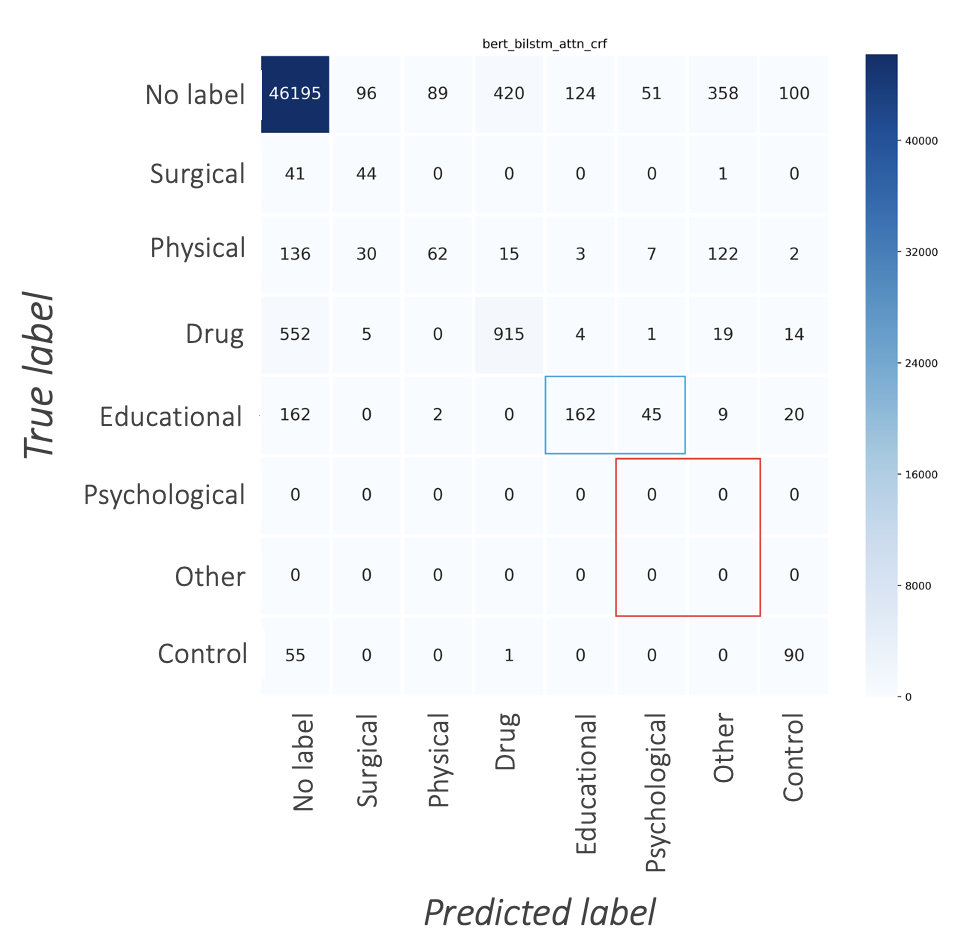
\includegraphics[scale=0.42]{figures/confusionmatrix.png}
    \caption{``Intervention'' entity example error matrix for the MTL experimental setup V (BERT BiLSTM attention CRF)}
    \label{fig:MTLexp1cm}
\end{figure}
%
The most obvious reason for this is the comparatively lower number of label annotations for these classes.
It was apparent during the manual annotation of the physiotherapy corpus that the ``Other'' entity encompassed any intervention mention that did not fall into the rest of ``Intervention'' classes making this class highly heterogeneous with a mixture of diverse entities that followed several patterns (see Table\ref{table:coarsefineconcept}).
Heterogeneous entities are a challenge for IR~\cite{jaseena2014issues}.

All the taggers were consistently confused between the physiological and educational intervention classes (see the blue box in Figure~\ref{fig:MTLexp1cm}), which are important for our field of interest.
This challenge is related to the ``Intervention'' class definition.
During manual annotation, it was rather difficult, even as a human annotator, whether to classify certain interventions as educational or psychological (for example, the psycho-educational intervention if administered by a psychologist is considered as psychological intervention and if administered by a nurse it is classified as an educational intervention).
The performance of automatic labeling was just a direct reflection of the difficulty emanating from class definitions.
General analysis of all the PICO confusion matrices shows several out-of-the-span entities were mislabelled as PICO and vice versa.
If it was merely PICO being miss-tagged as out-of-the-span, it could have pointed to the class-imbalance problem given that out-of-the-span forms the majority class.
However, consistently even the out-of-the-span entities were mislabelled as PICO which points to the class-overlap problem.
Error inspection showed that the overall limited performance of these classifiers might result from the class-overlap between the PICO and out-of-the-span classes and ambiguities in how each coarse-grained PICO was divided further into fine-grained PICO classes, especially for the health entities.
%
\section{Conclusion}
\label{sec:conclusion}
%
We propose two end-to-end neural model setups for fine-grained PICO recognition that outperform the previous SOTA for the fine-grained ``Participant'' and ``Outcome'' entities without any need for hand-engineered features.
We show that MTL is not only feasible but also a good alternative to the STL setup.
However, combining even the seemingly related tasks in MTL might not directly boost the performance.
To perform similar to or outperform its STL counterpart, MTL could require rather careful individual weighting of the involved tasks and task losses.
We contribute a manually annotated dataset with multi-level PICO annotations adding to the currently available resources.
Our error analysis warrants rethinking of semantically solid class definitions for fine-grained PICO entities along with ontology development for the health domain.
The code and the annotated in-house dataset are available on Github\footnote{\url{https://github.com/anjani-dhrangadhariya/multitask-pico-detection}}.
%
%
% ---- Bibliography ----
%
% BibTeX users should specify bibliography style 'splncs04'.
% References will then be sorted and formatted in the correct style.
%
\bibliographystyle{splncs04}
\bibliography{bibliography}
%
\end{document}